\chapter{Vision}\label{chap:vision}
Vision is one of the information-rich sensor system both humans and robots have available. Processing the wealth of information that is generated by vision sensors is still a key challenge, however. The goal of this chapter is to introduce
\begin{itemize}
\item images as two-dimensional signals,
\item providing an intuition of the wealth of information hidden in low-level information,
\item introducing basic convolution and threshold-based image processing algorithms.
\end{itemize}

\section{Images as two-dimensional signals}
Images are captured by cameras containing matrices of charge-coupled devices (CCD) or similar semi-conductors that can turn photons into electrical signals. These matrices can be read out pixel by pixel and turned into digital values, for example an array of 640 by 480 three-byte tuples corresponding to the red, green, and blue (RGB) components the camera has seen. An example of such data, for simplicity only one color channel, is shown in Figure \ref{fig:iss_closeup}. 

Looking at the data clearly reveals the white tile within the black tiles at the lower-right corner of the chessboard. Higher values correspond to brighter colors (white) and lower values to darker colors. We also observe that although the tiles have to have the same color, the actual values differ quite a bit. It might make sense to think about these values much like we would do if the data would be 1D signal: taking the ``derivative'', e.g., along the horizontal rows, would indicate areas of big changes, whereas the ``frequency'' of an image  would indicate how quickly values change. Areas with smooth gradients, e.g., black and white tiles, would then have low frequencies, whereas areas with strong gradients, would contain high frequency information. 

\begin{figure}[!htb]
	\centering
		\includegraphics[width=\textwidth]{figs/iss_closeupmatrix}
	\caption{A chessboard floating inside the ISS, astronaut Gregory Chamitoff. The inset shows a sample of the actual data recorded by the image sensor. One can clearly recognize the contours of the white tile.}
	\label{fig:iss_closeup}
\end{figure}

This language opens the door to a series of signal processing concepts, such as low-pass filters (supressing high frequency information), high-pass filters (suppressing low frequency information), or band-pass filters (letting only a range of frequencies pass), analysis of the frequency spectrum of the image (the distribution of content at different frequencies), or ``convolving'' the image with another two-dimensional function. The next sections will provide both an intuition of what kind of meaningful information is hidden in such abstract data and provide concrete examples of signal processing techniques that make this information appear.

\section{From signals to information}
Unfortunately, many phenomena that often have very different or even opposite meaning look very similar when looking at the low-level signal. For example, drastic changes in color values do not necessarily mean that the color of a surface indeed has changed. Similar patterns are generated by depth discontinuities, specular highlights, changing lighting conditions, or surface orientation changes. These examples are illustrated in Figure \ref{fig:iss_edges} and make computer vision a hard problem.  

\begin{figure}[!htb]
	\centering
		\includegraphics[width=\textwidth]{figs/iss_edges}
	\caption{Inside of the international space station (left), highlighted areas in which pixel values change drastically (right). Underlying effects that produce similar responses: change in surface properties (1), depth discontinuities (2), specular highlights (3), changing lighting conditions such as shadows (4), or surface orientation changes (5).
	\label{fig:iss_edges}}
\end{figure}

This example illustrates that signals alone are not sufficient to understand a phenomenon, but require context. Here, the context does not only refer to surrounding signals, but also high-level conceptional knowledge such as the fact that light sources create shadows and specular highlights, that objects in the front appear larger, and so on. How important such conceptional knowledge is, is illustrated by Figure \ref{fig:craters}.

Both images show an identical landscape that once appears to be speckled with craters, once with bubble-like hills. At first glance, both scenes are illuminated from the left, suggesting a change in the landscape. Once information that the sun is illuminating one picture from the left and the other from the right, however, it becomes clear that the craters are simply differently illuminated and what we perceive as bumps eventually turns back into craters. 

\begin{figure}[!htb]
	\centering
		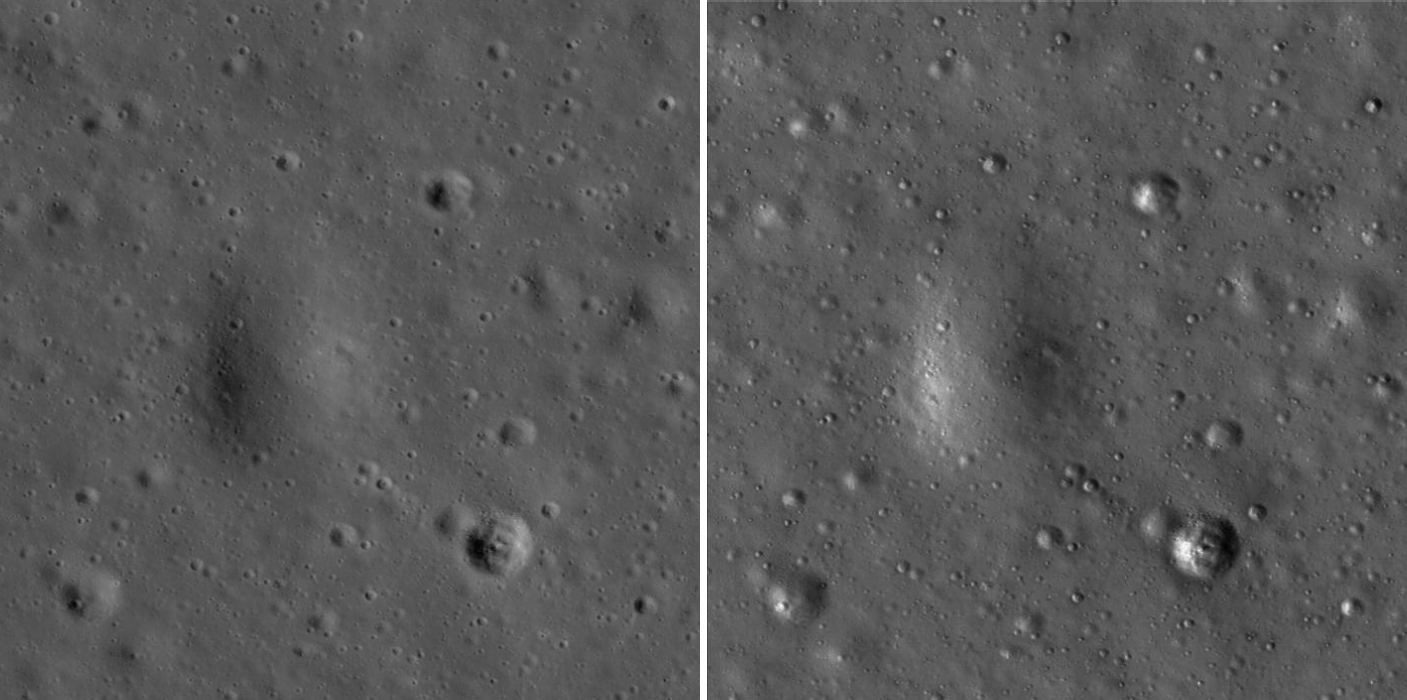
\includegraphics[width=\textwidth]{figs/craters}
	\caption{Picture of the Apollo 15 landing site during different times of the day. The landscape is identical, but appears to be speckled with craters (lift) or hills (right). Knowing that the sun is illuminating the scene from the left and right, respectively, does explain this effect. Image credit: NASA/GSFC/Arizona State University.
	\label{fig:craters}}
\end{figure}

More surprisingly, conceptual knowledge is often sufficient to make up for the lack of low-level cues in an image. An example is shown in Figure \ref{fig:dalmatian}. Here, a Dalmatian dog can be clearly recognized despite absence of cues for its outline, simply by extrapolating its appearance and pose from conceptual knowledge. 

These examples illustrate both the advantages and drawbacks of a signal processing approach. While an algorithm will detect interesting signals even there where we don't see, or don't expect them (due to conceptional bias), image understanding not only requires low-level processing, but intelligent combination of the low-level cue's spatial relationship and conceptual knowledge about the world. 


\begin{figure}
	\centering
		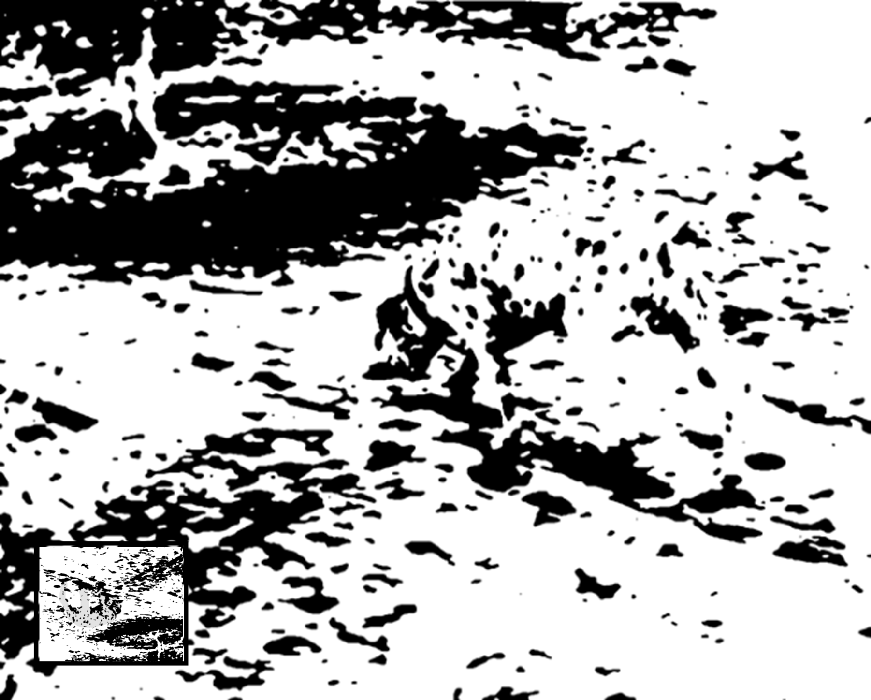
\includegraphics[width=\textwidth]{figs/dalmatian}
	\caption{The image of a Dalmatian dog can be clearly recognized by most spectators even though low-level cues such as edges are only present for ears, chin and parts of the legs. The contours of the animals are highlighted in a flipped version of the image in the inset.
	\label{fig:dalmatian}}
\end{figure}

\section{Basic image operations}
Basic image operations can be thought of as a filter that operates in the frequency or in the space (color) domain. Although most filters directly operate in the color domain, knowing how they affect the frequency domain is helpful in understanding the filter's function. For example, a filter that is supposed to highlight edges, such as shown in Figure \ref{fig:iss_edges} should suppress low frequencies, i.e., areas in which the color values do not change much, and amplify high-frequency information, i.e., areas in which the color values change quickly. The goal of this section is to provide a basic understanding of how basic image processing operation works. The methods presented here, while still valid, have been superseded by more sophisticated implementations that are widely available as software packages or within desktop graphic software.

\subsection{Convolution-based filters}
 A filter can be implemented using the \emph{convolution} \index{Convolution} operator that convolves function $f()$ with function $g()$. 
\begin{equation}
f(x)\star g(x)=\int_{-\infty}^{\infty}f(\tau)g(x-\tau)d\tau
\end{equation}
We then call function $g()$ a \emph{filter}\index{Filter}. As will become more clear further below, the convolution literally shifts the function $g()$ across the function $f()$ while multiplying the two. As images are discrete signals, the convolution is usually discrete
\begin{equation}
f[x]\star g[x]=\sum_{i=-\infty}^{\infty}f[i]g[x-i]
\end{equation} 
For 2D signals, like images, the convolution is also two-dimensional:
\begin{equation}\label{eq:2dconv1}
f[x,y]\star g[x,y]=\sum_{i=-\infty}^{\infty}\sum_{j=-\infty}^{\infty}f[i,j]g[x-i,y-j]
\end{equation}
Although we have defined the convolution from negative infinity to infinity, both images and filters are usually finite. Images are constrained by their resolution, and filters are usually much smaller than the images themselves. Also, the convolution is commutative, therefore (\ref{eq:2dconv1}) is equivalent to 
\begin{equation}\label{eq:2dconv2}
f[x,y]\star g[x,y]=\sum_{i=-\infty}^{\infty}\sum_{j=-\infty}^{\infty}f[x-i,y-j]g[i,j].
\end{equation}

\subsubsection{Gaussian smoothing}
A very important filter is the Gaussian filter.\index{Gaussian filter} It is shaped like the Gaussian bell function and can be easily stored in a 2D matrix. Implementing a Gaussian filter is surprisingly simple, e.g., such as
\begin{equation}
g(x,y)=\frac{1}{10}
\left(
\begin{array}{ccc}
1 & 1 & 1\\
1 & 2 & 1\\
1 & 1 & 1\\
\end{array}
\right)
\end{equation}
Using this filter in Equation \ref{eq:2dconv2} on an infinitely large image $f()$ leads to
\begin{equation}\label{eq:2dconv3}
f[x,y]\star g[x,y]=\sum_{i=-1}^{1}\sum_{j=-1}^{1}f[x-i,y-j]g[i,j]
\end{equation}
(assuming $g(0,0)$ addresses the center of the matrix). What now happens is that each pixel $f(x,y)$ becomes the average of that of its neighbors, with its previous value weighted twice (as $g(0,0)=0.2$) that of their neighbors. More concretely,
\begin{equation}
\tiny
f(x,y)=
\begin{array}{lll}
f(x+1,y+1)g(-1,-1) &+f(x+1,y)g(-1,0) &+f(x+1,y-1)g(-1,1)\\
+f(x,y+1)g(0,-1) &+f(x,y)g(0,0) &+f(x,y-1)g(0,1)\\
+f(x-1,y+1)g(1,-1) &+f(x-1,y)g(1,0) &+f(x-1,y-1)g(1,1)
\end{array}
\end{equation}
Doing this for all $x$ and all $y$ literally corresponds to sliding the filter $g()$ along the image. 

\begin{figure}
	\centering
		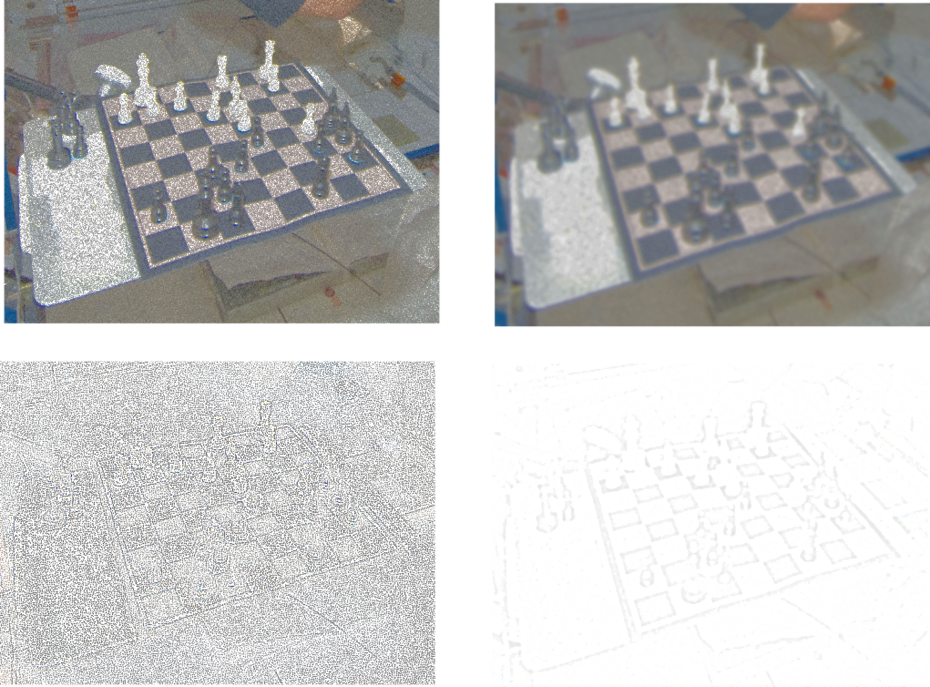
\includegraphics[width=\textwidth]{figs/filters}
	\caption{A noisy image before (top left) and after filtering with a Gaussian kernel (top right). Corresponding edge images are shown underneath. 
	\label{fig:filters}}
\end{figure}

An example of filter $g(x,y)$ in action is shown in Figure \ref{fig:filters}. The filter acts as a \emph{low-pass filter} \index{Low-pass filter}, suppressing high frequency components. Indeed, noise in the image is suppressed, leading also to a smoother edge image, which is shown underneath.

\subsubsection{Edge detection}\label{sec:sobel}
Edge detection can be achieved using another convolution-based filter, the \emph{Sobel} kernel\index{Sobel filter}
\begin{equation}
s_x(x,y)=
\left(
\begin{array}{ccc}
-1 & 0 & 1\\
-2 & 0 & 2\\
-1 & 0 & 1\\
\end{array}
\right)
\qquad
s_y(x,y)=
\left(
\begin{array}{ccc}
1 & 2 & 1\\
0 & 0 & 0\\
-1 & -2 & -1\\
\end{array}
\right)
\end{equation}
Here, $s_x(x,y)$ can be used to detect vertical edges, whereas $s_y(x,y)$ highlights horizontal edges. Edge detectors, such as the \emph{Canny} edge detector\index{Canny edge detector}  therefore run at least two of such filters over an image to detect both horizontal and vertical edges.

\subsubsection{Difference of Gaussians}
An alternative method for detecting edges is the \emph{Difference of Gaussians} (DoG) method \index{Difference of Gaussians (DoG)}. The idea is to subtract two images that have each been filtered using a Gaussian kernel with different width. Both filters supress high-frequency information and there difference therefore leads to a \emph{band-pass} filtered signal\index{Band-pass filter}, from which both low and high frequencies have been removed. As such, a DoG filter acts as a capable edge detection algorithm. Here, one kernel is usually four to five times wider than the other, therefore acting as a much stronger filter.

Differences of Gaussians can also be used to approximate the \emph{Laplacian of Gaussian},\index{Laplacian of Gaussian} i.e., the sum of the second derivatives of a Gaussian kernel. Here, one kernel is roughly 1.6 times wider than the other. The band-pass characteristic of DoG and LoGs are important as they highlight high-frequency information such as edges, yet suppress high-frequency noise in the image.


\subsection{Threshold-based operations}
In order to find objects with a certain color or edge intensity, tresholding an image will lead to a binary image that contains ``true-false'' regions that fit the desired criteria. Thresholds make use of operators like $>,<,\leq,\geq$ and combinations thereof. There also exist adaptive versions that would adapt the thresholds locally, e.g., to make up for changing lighting conditions.

Albeit thresholding is deceptively simple, finding correct threshold values is a hard problem. In particular, actual pixel values change drastically with changing lighting conditions and there is no such thing as ``red'' or ``green'' when inspecting the actual values under different conditions. 

\subsection{Morphological Operations}
Another class of filters are morphological operators which consists of a kernel describing the structure of the operation (this can be as simple as an identity matrix) and a rule on how to change a pixel value based on the values in the neighborhood defined by the kernel.

Important morphological operators are \emph{erosion} and \emph{dilation} \index{Erosion}\index{Dilation}. The erosion operator assigns a pixel value with the minimum value that it can find in the neighborhood defined by the kernel. The dilation operator assigns a pixel value with the maximum value it can find in the neighborhood defined by the kernel. This is useful, e.g., to fill holes in a line or remove noise. A dilation followed by an erosion is known as a ``Closing'' and an erosion followed by a dilation as an ``Opening''. Subtracting erosed and dilated images from each other can also serve as an edge detector. Examples of such operators are shown in Figure \ref{fig:morphology}.

\begin{figure}
	\centering
		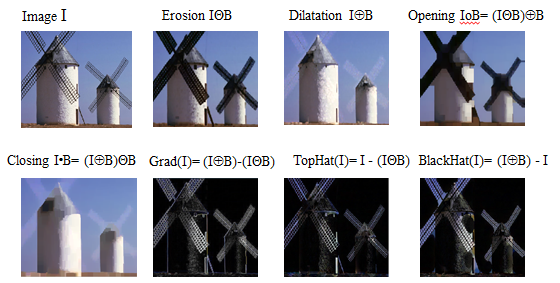
\includegraphics[width=\textwidth]{figs/morphology}
	\caption{Examples of morphological operators erosion and dilation and combinations thereof.
	\label{fig:morphology}}
\end{figure}


\section*{Exercises}\small
\begin{enumerate}
\item Below are shown multiple ``Kernels'' that can be used for convolution-based image filtering. 
\begin{equation}
\nonumber
\begin{array}{|c|c|c}
\hline
1 & 1 & 1\\
\hline
1 & 2 & 1\\
\hline
1 & 1 & 1
\end{array}
\quad
\begin{array}{|c|c|c}
\hline
0 & -1 & 0\\
\hline
0 & -1 & 0\\
\hline
0 & -1 & 0
\end{array}
\quad
\begin{array}{|c|c|c}
\hline
1 & 1 & 1\\
\hline
1 & -4 & 1\\
\hline
1 & 1 & 1
\end{array}
\end{equation}
\begin{enumerate}
\item Identify the Kernel, which can blur an image.
\item What kind of features can be detected by the other two kernels?
\end{enumerate} 
\end{enumerate} \normalsize